
% ------------------------------------------------------------
\section{Three microscopic stories for \texorpdfstring{$\kappa(D(0))$}{kappa(D(0))}}
\label{sec:kappa-stories}
% ------------------------------------------------------------

The monotonicity just derived held with $\kappa$ treated as a fixed parameter.
Physically, however, the trap reactivity can depend on the local mobility:
whether the $1/\kappa$ dwell time grows or shrinks with $D(0)$ depends on the
microscopic mechanism by which the particle detects the target.  We compare
three canonical scenarios:
\begin{enumerate}[label=(\Roman*)]
\item \textbf{$\kappa$ independent of $D(0)$.}  The standard assumption.  The
   decomposition \eqref{eq:T-avg-general} is fully additive.  As shown above,
   $\langle T\rangle$ decreases monotonically with $D_1$.
\item \textbf{$\kappa=\kappa_0\,D(0)$.}  Faster motion at the trap increases the
   encounter rate: more collisions per unit time means higher reactivity.
   The dwell time becomes $2\pi/(\kappa_0\,D(0))$, which \emph{also} decreases with
   $D_1>0$.  Both terms drive $\langle T\rangle$ down with increasing $D_1$:
   there is no interior optimum.
\item \textbf{$\kappa=\kappa_0/D(0)$.}  Slower motion at the trap enhances
   recognition: the detector requires a minimum contact time to register the
   target (a bee must slow down to identify the food source).  Now the dwell
   time is $2\pi\,D(0)/\kappa_0$, which \emph{grows} with $D_1$ and competes
   against the decreasing travel contribution.  A non-trivial optimum $D_1^*$
   exists.
\end{enumerate}
The qualitative behaviour of the three stories on the tent profile is
displayed in Figure~\ref{fig:kappa-stories} (generated numerically from
\eqref{eq:T-avg-tent}).

\begin{figure}[!ht]
\centering
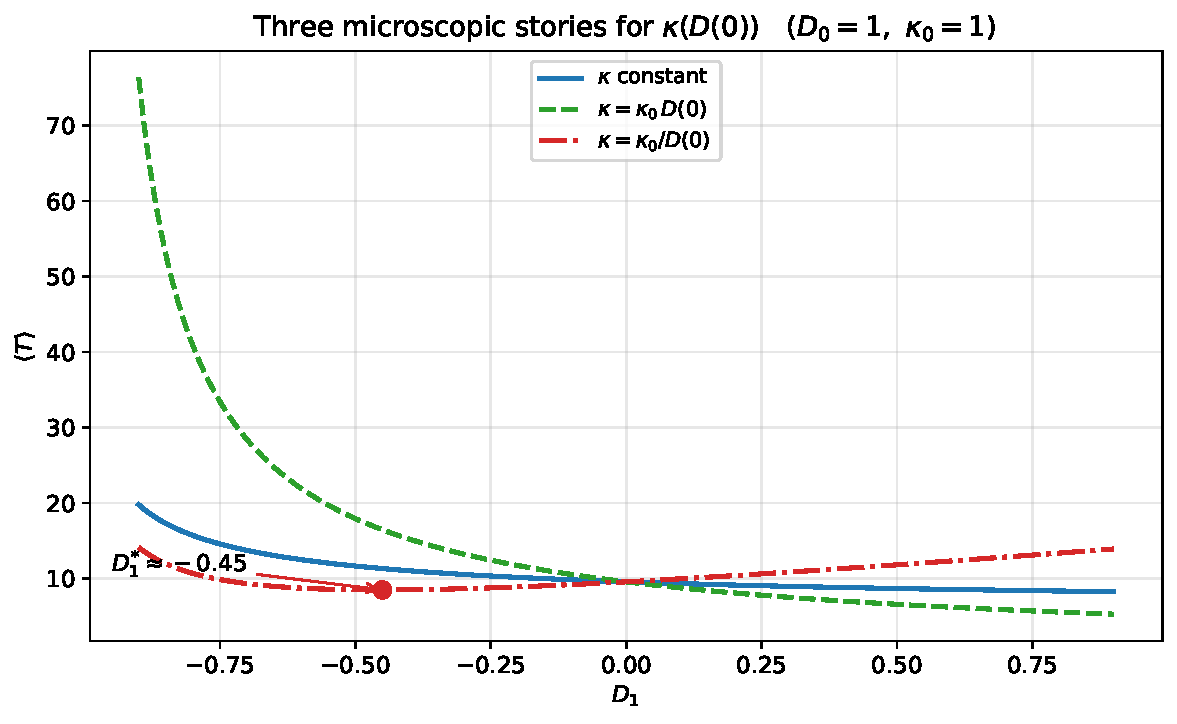
\includegraphics[width=0.7\linewidth]{files/fig_kappa_stories.pdf}
\caption{The three microscopic stories for $\kappa(D(0))$ applied to the tent
profile with $D_0=1$ and $\kappa_0=1$.  Only the $1/D(0)$ story
(red, dash-dotted) exhibits an interior optimum $D_1^*$; the other two are
monotone.  The marked point indicates the numerically determined minimum.}
\label{fig:kappa-stories}
\end{figure}

For story (III) the optimum $D_1^*$ satisfies
\[
\frac{\partial\langle T\rangle}{\partial D_1}\bigg|_{D_1^*}
=\frac{2\pi}{\kappa_0}
-\frac{1}{\pi}\int_0^\pi\!\frac{(\pi-y)^2\,(1-y/\pi)}{D(y)^2}\,dy
\Bigg|_{D_1^*}
=0,
\]
whose numerical solution with $D_0=\kappa_0=1$ gives
$D_1^*\approx -0.45$ (see Section~\ref{sec:results}).
The sign is physically sensible: with $\kappa=\kappa_0/D(0)$ the dwell time
$2\pi D(0)/\kappa_0$ \emph{decreases} when $D_1<0$ (a dip at the trap), so the
optimum sits in the negative-$D_1$ region, i.e.\ the food source is best
placed in a congested part of the nest where the bee spends enough time to
register it.
